\documentclass[tikz,multi]{standalone}

\usepackage{tikzducks}
\usepackage{duckuments}

\begin{document}
\makeatletter
\foreach\x in {1,2,...,\duckuments@randoms}
  {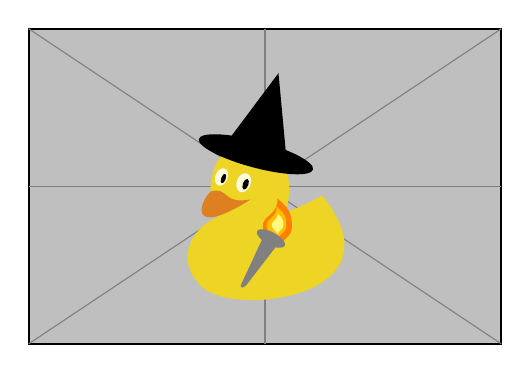
\begin{tikzpicture}
    \draw[black,fill=gray!50,thick] (0,0) rectangle (6,4);
      \draw[gray] (0,0) -- (6,4);
      \draw[gray] (0,4) -- (6,0);
      \draw[gray] (3,0) -- (3,4);
      \draw[gray] (0,2) -- (6,2);
      \node at (3,2) {\tikz\randuck;};
  \end{tikzpicture}}
\makeatother
\end{document}
